
% This LaTeX was auto-generated from MATLAB code.
% To make changes, update the MATLAB code and republish this document.

\documentclass{article}
\usepackage{graphicx}
\usepackage{color}

\sloppy
\definecolor{lightgray}{gray}{0.5}
\setlength{\parindent}{0pt}

\begin{document}

    
    
\subsection*{Contents}

\begin{itemize}
\setlength{\itemsep}{-1ex}
   \item Read ROIs from The Crick
   \item display 1 slice of 1 data set
\end{itemize}


\subsection*{Read ROIs from The Crick}

\begin{verbatim}
dir0                = dir('*.tiff');
\end{verbatim}


\subsection*{display 1 slice of 1 data set}

\begin{verbatim}
currentSet          = 12;
currentName         = dir0(currentSet).name;
currentSetInfo      = imfinfo(dir0(currentSet).name);
numSlices           = size(currentSetInfo,1);

filtG               = gaussF(5,5,1);
\end{verbatim}
\begin{verbatim}
%currentSlice=242;
centralSlice        = round(numSlices/2);
currentImage        = imread(dir0(currentSet).name,centralSlice);
figure(1)
imagesc(imfilter(currentImage,filtG))
title(strcat(dir0(currentSet).name,'  (',num2str(currentSet),')    ','   -  ',num2str(centralSlice),'/',num2str(numSlices)),'interpreter','none')
colormap gray
Hela_nuclei(:,:,centralSlice) = segmentNucleiHelaEM(currentImage);
Hela_background(:,:,centralSlice) = segmentBackgroundHelaEM(currentImage);

figure(2)
imagesc( Hela_nuclei(:,:,centralSlice));

colormap gray
\end{verbatim}

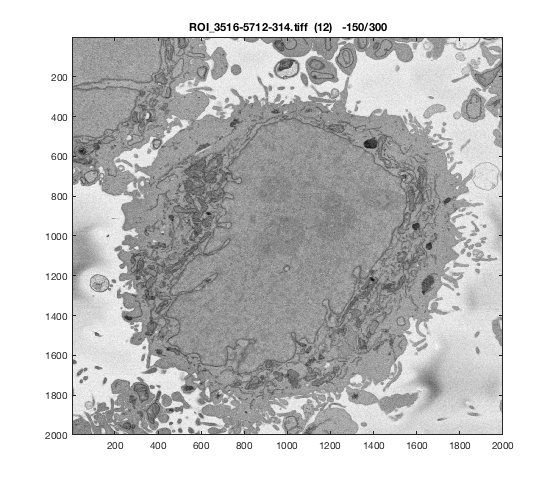
\includegraphics [width=4in]{testGit_01.eps}

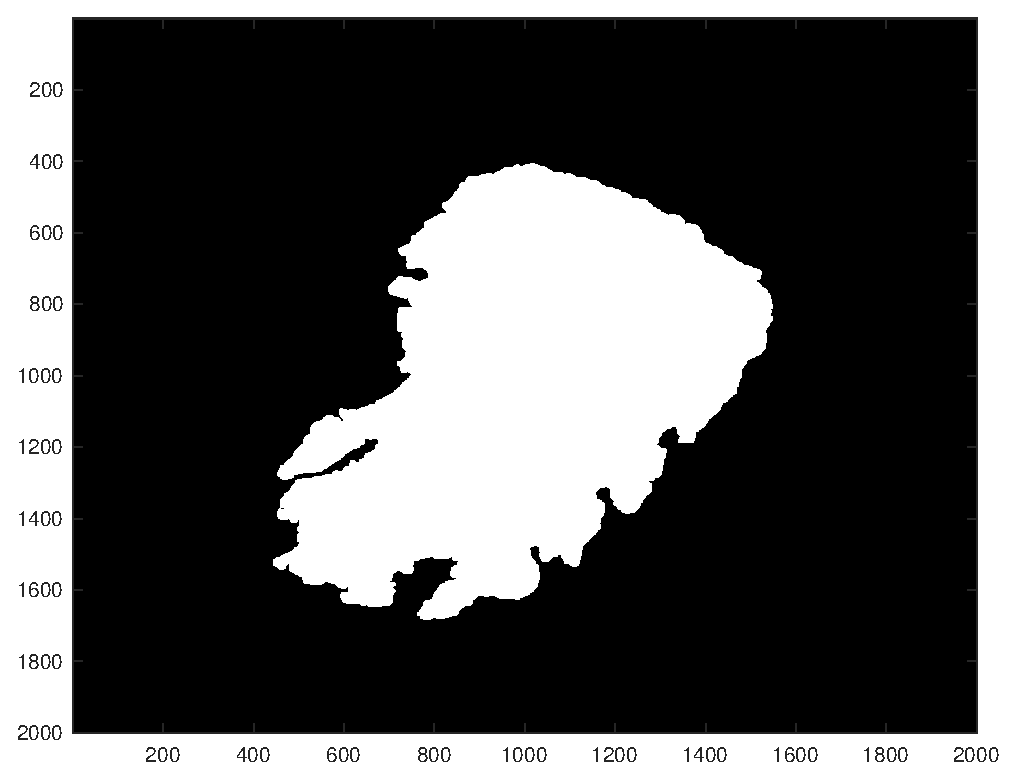
\includegraphics [width=4in]{testGit_02.eps}



\end{document}
    
